% ACL 2025 LaTeX paper — Fine-tune GLM-OCR for Vietnamese OCR
% Compile on Overleaf: select pdfLaTeX compiler
\documentclass[11pt]{article}

% ACL style
\usepackage{acl}
\usepackage{times}
\usepackage{latexsym}
\usepackage[T1]{fontenc}
\usepackage[utf8]{inputenc}
\usepackage{microtype}
\usepackage{inconsolata}
\usepackage{graphicx}
\usepackage{booktabs}
\usepackage{multirow}
\usepackage{amsmath}
\usepackage{amssymb}
\usepackage{hyperref}
\usepackage{xcolor}
\usepackage{enumitem}
\usepackage{caption}

% Vietnamese support
\usepackage[vietnamese]{babel}

\hypersetup{
    colorlinks=true,
    linkcolor=blue!60!black,
    citecolor=blue!60!black,
    urlcolor=blue!60!black
}

\title{Research on Lightweight MLLM for Vietnamese OCR:\\
Fine-tuning GLM-OCR for Diacritical Mark Recognition}

\author{
  Tuan Dung Nguyen \quad Trong Kien Nguyen \quad Nhat Linh Pham \\
  Faculty of Computer Science, University of Information Technology \\
  Vietnam National University - Ho Chi Minh City \\
  \texttt{\{dung.nguyentuan, kien.nguyentrong, linh.phamnhat\}@uit.edu.vn}
}

\date{}

\begin{document}

\maketitle

% ============================================================
\begin{abstract}
Vietnamese is a tonal language with a complex diacritical system comprising six tones and multiple double-diacritical characters (ă, â, ê, ô, ơ, ư, đ). 
Existing Vision-Language Models (VLMs) for OCR, including GLM-OCR (0.9B parameters), struggle to accurately recognize these diacritical marks due to insufficient Vietnamese training data. 
In this paper, we present a comprehensive fine-tuning pipeline for GLM-OCR targeting Vietnamese diacritical mark recognition. 
Our approach employs a two-stage curriculum learning strategy: Stage 1 uses 50K synthetic line-level images generated from a curated Vietnamese dictionary with 14 augmentation types, while Stage 2 uses 10K document-level images crawled from Vietnamese news sources. 
We introduce an anti-bias mechanism combining plain-word injection and diacritic stripping to prevent the model from hallucinating diacritics on plain text. 
Our evaluation framework includes diacritic accuracy per group and a novel false positive rate metric. 
The resulting models are deployed via Ollama for practical use.
\end{abstract}

% ============================================================
\section{Introduction}

Optical Character Recognition (OCR) has undergone a paradigm shift with the emergence of Vision-Language Models (VLMs). 
Traditional OCR systems such as Tesseract \cite{smith2007ocr} and PaddleOCR \cite{paddleocr2022} rely on multi-stage pipelines (text detection $\rightarrow$ segmentation $\rightarrow$ recognition) that struggle with complex layouts and non-Latin scripts. 
Modern VLMs treat document understanding as a unified semantic task, processing entire pages end-to-end to generate structured outputs.

However, Vietnamese poses unique challenges for OCR systems. 
The language employs six tones (ngang, sắc, huyền, hỏi, ngã, nặng) and numerous double-diacritical characters (ă, â, ê, ô, ơ, ư, đ), resulting in over 160 unique letter-tone combinations. 
A single diacritical mark can completely change word meaning: ``ma'' (ghost), ``má'' (mother), ``mà'' (conjunction), ``mả'' (tomb), ``mã'' (code), ``mạ'' (rice seedling) --- six words differentiated only by tone marks. 
This makes diacritical accuracy not merely a cosmetic concern but a semantic necessity.

Current VLMs, including GLM-OCR \cite{glm-ocr} from Zhipu AI, achieve strong performance on English and Chinese OCR but poorly recognize Vietnamese diacritics. 
The primary cause is the absence of high-quality Vietnamese training data in pre-training corpora. 
Fine-tuning is therefore essential, but full fine-tuning of even a 0.9B model is prohibitively expensive on consumer hardware.

In this paper, we present a complete fine-tuning pipeline for GLM-OCR targeting Vietnamese diacritical mark recognition. 
Our contributions are:
\begin{enumerate}[nosep,leftmargin=*]
    \item A synthetic data generation system with 14 augmentation types, 58 verified fonts, and 7 sample generators including confusion pairs and anti-bias plain words.
    \item A two-stage curriculum learning approach transitioning from synthetic line-level data to real-world document-level news data.
    \item A dual-layer anti-bias mechanism to prevent diacritical hallucination, measured by a novel false positive rate metric.
    \item A comprehensive evaluation framework including per-group diacritic accuracy across 7 character groups.
    \item Deployment tooling via LoRA merging and Ollama for practical inference.
\end{enumerate}

% ============================================================
\section{Related Work}

\subsection{VLMs for Document Understanding}

The field of document understanding has evolved through three distinct phases.

\textbf{Traditional OCR} systems (2010s) follow pipeline-based architectures: text detection (e.g., CTPN, EAST), followed by segmentation and character recognition (CRNN with CTC loss). 
Tesseract \cite{smith2007ocr} and PaddleOCR \cite{paddleocr2022} are representative systems that perform well on printed English text but struggle with complex layouts, handwriting, and non-Latin scripts.

\textbf{Generalist VLMs} (2023--2024) such as Qwen2.5-VL \cite{qwen2vl}, GPT-4o, Gemini 2.0 Flash, and InternVL2 \cite{internvl2024} treat OCR as a semantic understanding task. 
These models process entire document images and generate structured text outputs, but their large size (7B--70B parameters) makes them impractical for edge deployment.

\textbf{Specialized OCR VLMs} (2025--2026) optimize specifically for document understanding with compact architectures: GLM-OCR (0.9B) \cite{glm-ocr}, OlmOCR-2 (8B), and dots.ocr (3B). 
These models achieve competitive accuracy at a fraction of the computational cost, making them ideal candidates for fine-tuning on domain-specific languages.

\subsection{Parameter-Efficient Fine-Tuning}

Full fine-tuning of large models requires updating billions of parameters, consuming significant GPU memory. 
LoRA \cite{hu2022lora} addresses this by injecting trainable low-rank matrices $\Delta W = BA$ where $A \in \mathbb{R}^{d \times r}$ and $B \in \mathbb{R}^{r \times k}$ with $r \ll \min(d,k)$, reducing trainable parameters from billions to millions while maintaining performance comparable to full fine-tuning. 
QLoRA \cite{dettmers2024qlora} further combines 4-bit quantization with LoRA for even lower memory usage.

We build on LoRA using the LLaMA-Factory \cite{llamafactory2024} framework, which provides a unified interface for efficient fine-tuning of 100+ language models with flexible freeze/unfreeze control over individual components.

\subsection{Curriculum Learning for OCR}

Multi-stage training has proven effective for OCR tasks. 
VARY \cite{vary2024} uses a two-process scheme with different resolutions for document parsing. 
TrOCR \cite{trocr2023} pre-trains on large-scale synthetic data before fine-tuning on real data. 
Monkey \cite{monkey2024} employs a multi-scale approach with progressive resolution enhancement. 
These approaches inspire our two-stage curriculum design: starting with simple, clean synthetic data before progressing to complex, noisy real-world data.

% ============================================================
\section{GLM-OCR Architecture}

GLM-OCR \cite{glm-ocr} is a 0.9B-parameter multimodal model specifically designed for document understanding. 
As shown in Figure~\ref{fig:architecture}, it takes a document image as input and processes it through three main components:

\begin{figure}[t]
    \centering
    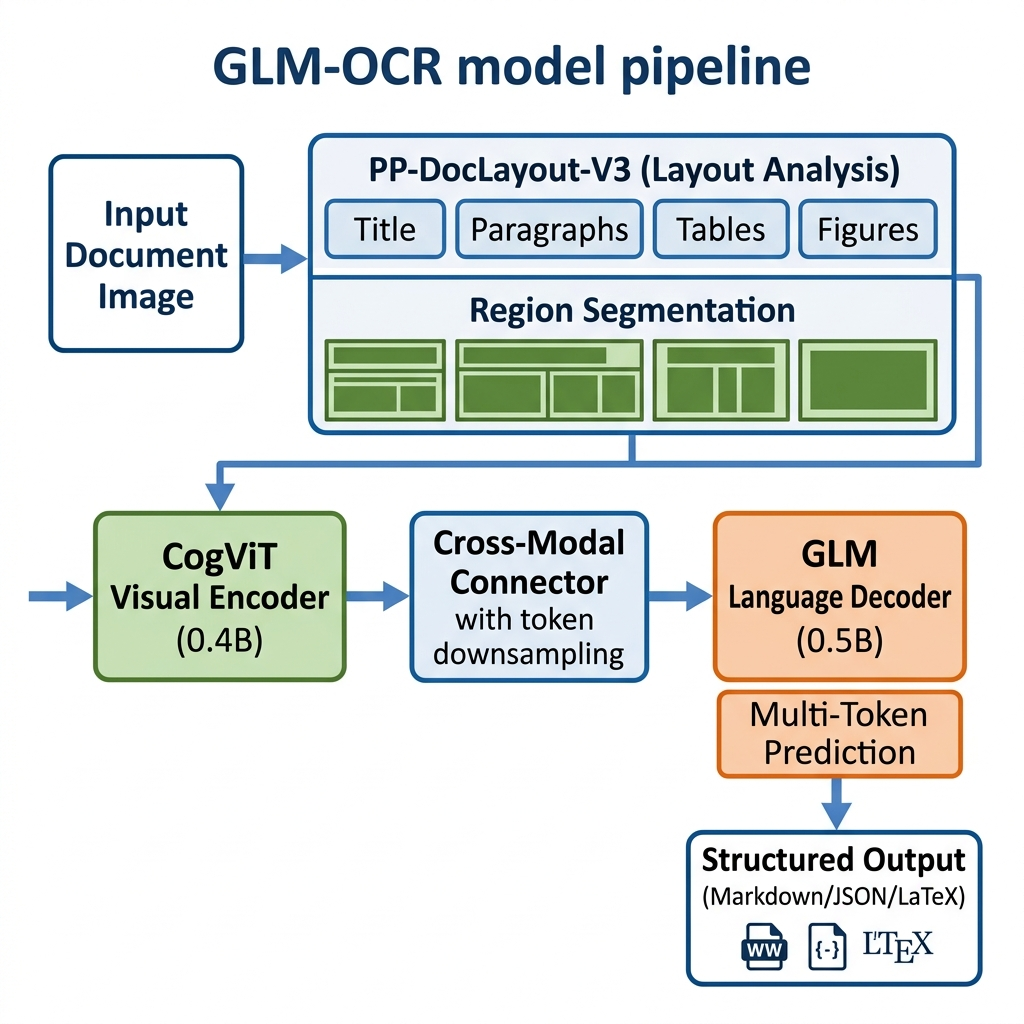
\includegraphics[width=\columnwidth]{glm_ocr_architecture.png}
    \caption{GLM-OCR architecture: Document image $\rightarrow$ PP-DocLayout-V3 layout analysis $\rightarrow$ CogViT visual encoder $\rightarrow$ Cross-modal connector $\rightarrow$ GLM decoder with Multi-Token Prediction $\rightarrow$ structured output.}
    \label{fig:architecture}
\end{figure}

\subsection{Visual Encoder (CogViT)}

The visual encoder is a 0.4B-parameter backbone based on the CogViT architecture with 24 transformer layers, hidden dimension 1024, and 16 attention heads. 
It processes input images at 336$\times$336 resolution using a patch size of 14$\times$14 with spatial merge size 2, producing approximately 999 visual tokens. 
The encoder is pre-trained on large-scale vision tasks and captures robust visual features including stroke patterns and spatial relationships.

\subsection{Cross-Modal Connector}

The connector maps visual tokens from the encoder's output space into the language model's embedding space. 
It performs token downsampling to reduce the visual sequence length before passing it to the decoder. 
This component is critical for fine-tuning because it must learn to map visual representations of Vietnamese diacritical marks to appropriate language tokens.

\subsection{Language Decoder}

The decoder is a 0.5B-parameter GLM (General Language Model) with 16 layers, hidden dimension 1536, and Grouped Query Attention (GQA) with 8 KV heads. 
Its vocabulary contains 59,392 tokens, which already includes common Vietnamese syllables. 
However, complex Vietnamese words like ``Nguyễn'' are split into 2--3 tokens, requiring the projector to map visual features across multiple token positions.

A key innovation is the Multi-Token Prediction (MTP) mechanism, which predicts multiple tokens per forward pass, achieving 5.2 tokens/step --- approximately 50\% faster than standard autoregressive decoding.

\begin{table}[t]
\centering
\small
\begin{tabular}{@{}ll@{}}
\toprule
\textbf{Component} & \textbf{Specification} \\
\midrule
Visual Encoder & 24 layers, $d$=1024, patches 14$\times$14 \\
Connector & Visual$\rightarrow$Language mapping \\
Language Decoder & 16 layers, $d$=1536, 16 heads \\
KV Heads (GQA) & 8 \\
Vocabulary & 59,392 tokens \\
Total Parameters & $\sim$0.9B \\
\bottomrule
\end{tabular}
\caption{GLM-OCR model specifications.}
\label{tab:specs}
\end{table}

% ============================================================
\section{Method}

\subsection{LoRA Configuration}

We apply LoRA with rank $r{=}16$, $\alpha{=}32$, dropout 0.1 to all linear layers (q/k/v/o\_proj, gate/up/down\_proj, lm\_head), yielding approximately 7.5M trainable parameters --- only 0.68\% of the total model parameters.

\begin{figure}[t]
    \centering
    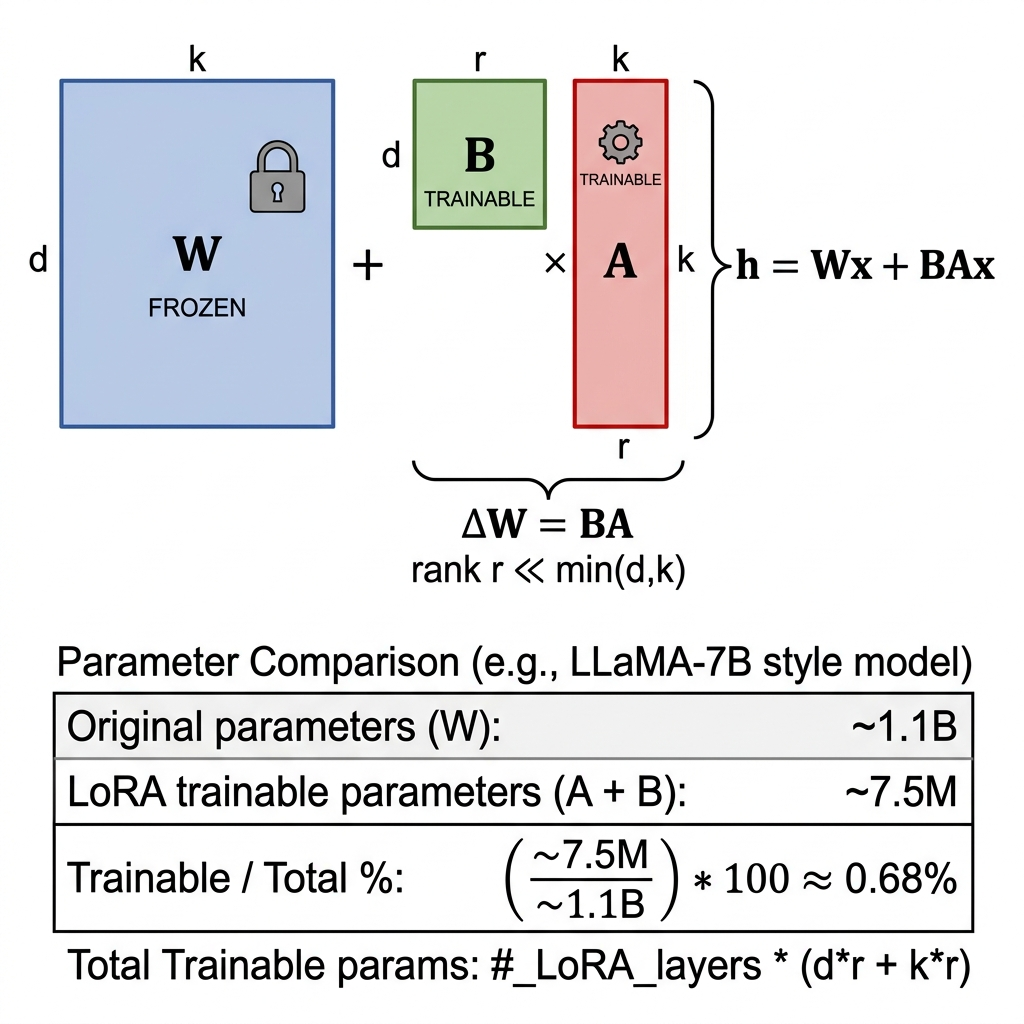
\includegraphics[width=0.85\columnwidth]{lora_architecture.png}
    \caption{LoRA architecture: $h = Wx + \Delta W x = Wx + BAx$ where $W$ is frozen and $A \in \mathbb{R}^{d \times r}$, $B \in \mathbb{R}^{r \times k}$ are trainable low-rank matrices.}
    \label{fig:lora}
\end{figure}

\textbf{Key design decision:} We freeze the visual encoder while \emph{unfreezing} the cross-modal projector. 
The rationale is twofold: (1) the pre-trained visual encoder already captures robust stroke and shape features that generalize across languages, and (2) unfreezing the projector allows it to learn new ``visual dictionary'' mappings specifically for Vietnamese diacritical patterns without degrading pre-trained visual capabilities. 
This strategy is critical because Vietnamese diacritics (combining horn, breve, circumflex, and tone marks) create visual patterns not well-represented in the original training data.

\subsection{Two-Stage Curriculum Learning}

Figure~\ref{fig:pipeline} illustrates our two-stage training pipeline.

\begin{figure}[t]
    \centering
    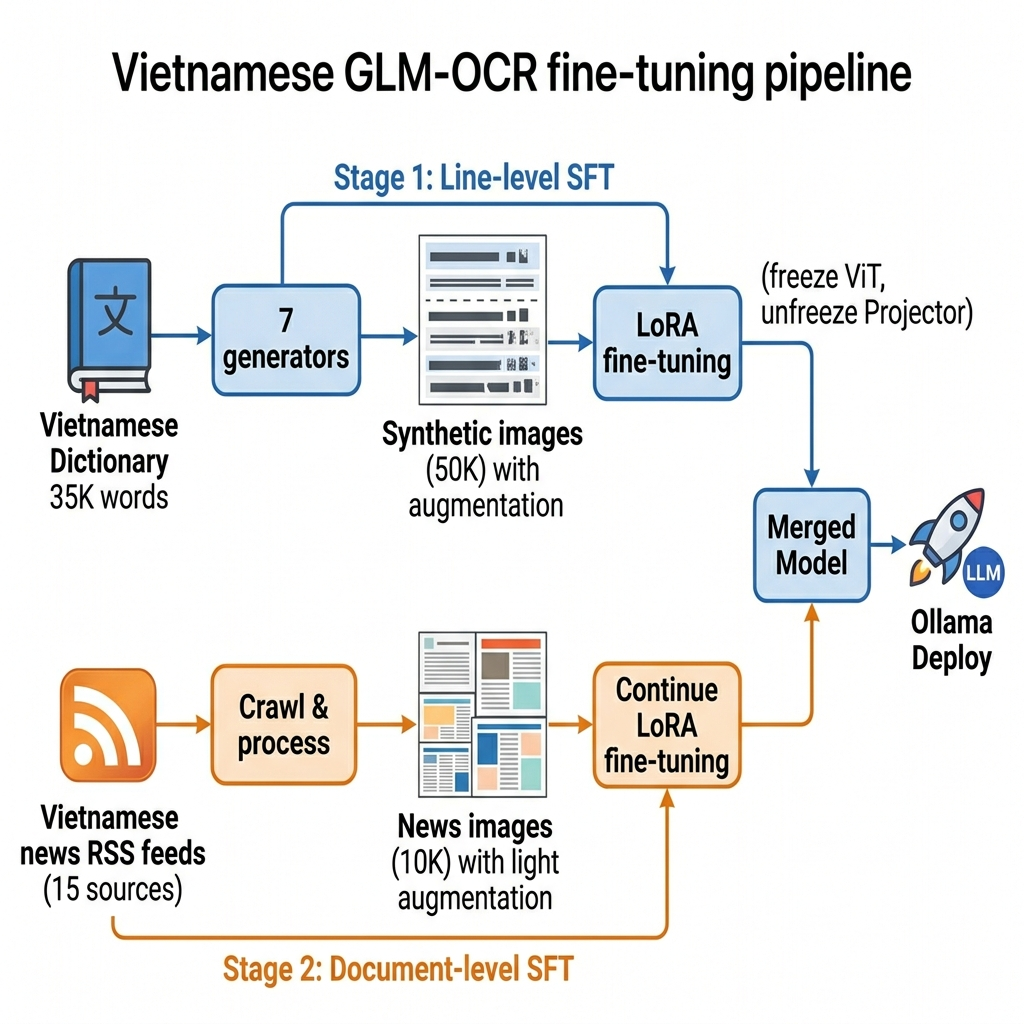
\includegraphics[width=\columnwidth]{finetune_pipeline.png}
    \caption{Two-stage fine-tuning pipeline for Vietnamese GLM-OCR. Stage 1 uses synthetic line-level data with diverse augmentation; Stage 2 uses crawled news data with anti-bias diacritic stripping.}
    \label{fig:pipeline}
\end{figure}

\paragraph{Stage 1: Line-Level SFT} 
Uses 50K synthetic images of short text lines (6--8 words per line). 
The model learns basic diacritical recognition with the projector unfrozen, establishing the visual-to-language mapping for Vietnamese characters. 
Configuration: LR=$10^{-4}$, constant\_with\_warmup (5\% warmup), effective batch=64, cutoff=2048, FP16 on T4.

\paragraph{Stage 2: Document-Level SFT} 
Loads the Stage 1 adapter (with optimizer state reset) and continues training on 10K news images with longer, more complex text. 
The lower learning rate and longer cutoff allow the model to refine its understanding on real-world data. 
Configuration: LR=$5 \times 10^{-5}$, effective batch=16, cutoff=4096, early stopping with patience=3.

The curriculum design follows the principle of progressive difficulty: Stage 1 provides clean, controlled examples to establish basic recognition, while Stage 2 exposes the model to real-world noise, varied layouts, and natural text flow.

\subsection{Vietnamese Dictionary Curation}

We curated a comprehensive Vietnamese dictionary from 36,534 original words. 
After cleaning (removing duplicates, non-Vietnamese entries, and proper nouns), we retained 35,501 clean words. 
We further identified 3,544 ``hard words'' containing double diacritics (e.g., ``nguời'', ``thuỷ'') through automated filtering of 20,378 candidates followed by manual verification.

The \texttt{filter\_vietnamese.py} module classifies words into 7 diacritic groups (ă, â, ê, ô, ơ, ư, đ) and generates up to 5,000 confusion pairs --- word pairs with edit distance = 1 that differ only in diacritical marks (e.g., ``chuổng'' vs.\ ``chuổng'', ``lặng'' vs.\ ``lẫm''). 
These pairs serve as challenging training samples to improve fine-grained diacritical discrimination.

\subsection{Synthetic Data Generation (Stage 1)}

The \texttt{generate\_vietnamese\_dataset\_v3.py} module generates diverse training data using 58 verified Windows fonts and 7 sample generators (Table~\ref{tab:generators}).

\begin{table}[t]
\centering
\small
\resizebox{\columnwidth}{!}{%
\begin{tabular}{@{}clp{3.8cm}@{}}
\toprule
\textbf{\#} & \textbf{Generator} & \textbf{Description} \\
\midrule
1 & gen\_word\_list (10\%) & 8--16 random words per line \\
2 & gen\_phrase\_list (25\%) & 2--4 phrases joined by commas \\
3 & gen\_confusion\_pair (15\%) & Minimal pairs with edit dist=1 \\
4 & gen\_grouped\_words (10\%) & Words from same diacritic group \\
5 & gen\_mixed\_line (15\%) & Phrases + individual words, multi-line \\
6 & gen\_dense\_sentence (25\%) & Dense sentences with periods \\
7 & gen\_plain\_words (10\%) & \textbf{Anti-bias}: mixed with/without diacritics \\
\bottomrule
\end{tabular}%
}
\caption{Seven sample generators for Stage 1 synthetic data.}
\label{tab:generators}
\end{table}

Each generator produces both an image and a ground-truth text file. 
Images are rendered on white backgrounds with randomized positioning, padding, and font size (24--48px). 
The \texttt{meta.json} protocol records split counts for reproducibility.

\subsection{News Crawling (Stage 2)}

The \texttt{crawl\_vi\_news.py} module collects real-world Vietnamese text from 15 RSS feeds across three major news sources: VNExpress (11 categories including technology, science, education), Tuổi Trẻ (4 categories), and Thanh Niên (1 category). 
Articles are extracted, filtered (length $>$ 50 characters, $>$ 60\% alphabetic ratio), and chunked into 2--10 line segments.

\textbf{30\% diacritic stripping:} Using Unicode NFD decomposition followed by combining mark removal, diacritics are stripped from 30\% of text chunks. 
This teaches the model \emph{not} to add diacritics where none exist in the source image --- a critical anti-hallucination strategy for production use.

\subsection{Data Augmentation}

14 augmentation types are applied to 60\% of training samples, while 40\% are kept clean to ensure the model learns diacritical patterns from uncorrupted images.

\begin{table}[t]
\centering
\scriptsize
\resizebox{\columnwidth}{!}{%
\begin{tabular}{@{}llll@{}}
\toprule
\textbf{Type} & \textbf{Params} & \textbf{Type} & \textbf{Params} \\
\midrule
Gaussian Blur & R 0.3--0.8 & Shadow & 5 directions \\
Gaussian Noise & I 15--35 & Glare & Bright overlay \\
Contrast $\uparrow$ & 1.1--1.5$\times$ & Perspective & 2--7\% warp \\
Contrast $\downarrow$ & 0.65--0.9$\times$ & Downscale & 0.75--0.92$\times$ \\
JPEG Compress & Q 55--80 & Wave & 2--10px sinusoid \\
Rotation & $\pm$3$^\circ$ & Elastic & $\sigma$=3--6 \\
Motion Blur & 5--12px & Defocus & Blur + noise \\
\bottomrule
\end{tabular}%
}
\caption{14 augmentation types with parameters. Stage 2 uses only 4 lighter types: blur, noise, JPEG, rotation.}
\label{tab:augmentation}
\end{table}

The augmentation pipeline simulates real-world image degradation: camera blur (Gaussian, motion, defocus), compression artifacts (JPEG), lighting variations (contrast, glare, shadow), geometric distortion (rotation, perspective, wave, elastic), and resolution loss (downscale). 
Stage 2 uses only 4 lighter augmentation types (blur, noise, JPEG, rotation) to avoid over-distorting real document images.

% ============================================================
\section{Training}

\subsection{Stage 1 Configuration}

\begin{table}[t]
\centering
\small
\resizebox{\columnwidth}{!}{%
\begin{tabular}{@{}lcc@{}}
\toprule
\textbf{Parameter} & \textbf{Stage 1} & \textbf{Stage 2} \\
\midrule
Learning Rate & $10^{-4}$ & $5 \times 10^{-5}$ \\
LR Scheduler & constant\_with\_warmup & constant\_with\_warmup \\
Warmup Ratio & 5\% & 5\% \\
Effective Batch Size & 64 (8 $\times$ 8 accum) & 16 (2 $\times$ 8 accum) \\
Cutoff Length & 2048 & 4096 \\
LoRA Rank ($r$) & 16 & 16 \\
LoRA Alpha ($\alpha$) & 32 & 32 \\
LoRA Dropout & 0.1 & 0.1 \\
Freeze ViT & Yes & Yes \\
Freeze Projector & No (unfrozen) & No (unfrozen) \\
Optimizer & AdamW (betas=0.9, 0.999) & AdamW (reset from S1) \\
Precision & FP16 & FP16 \\
Early Stop Patience & 3 & 3 \\
Dataset Size & 50,000 & 10,000 \\
VRAM Usage & $\sim$6.9 GB & $\sim$7.2 GB \\
\bottomrule
\end{tabular}%
}
\caption{Complete training hyperparameters for both stages.}
\label{tab:training}
\end{table}

We use the \texttt{constant\_with\_warmup} scheduler rather than cosine annealing for an important practical reason: cosine schedules decay the learning rate to near-zero by the end of training, making it difficult to resume across Colab sessions. 
With constant\_with\_warmup, the learning rate returns to its full value after warmup, enabling seamless resumption.

The training notebook auto-detects the latest checkpoint on Google Drive and computes the starting epoch number, eliminating manual configuration when resuming interrupted training sessions.

\subsection{Anti-Bias Strategy}

Diacritical hallucination --- where the model incorrectly adds diacritics to plain text --- is a critical failure mode for Vietnamese OCR. 
We address this through a dual-layer mechanism:

\begin{enumerate}[nosep]
    \item \textbf{gen\_plain\_words (10\% of Stage 1):} Injects text lines containing words both with and without diacritics, explicitly teaching the model that plain Latin characters are valid and should not be modified.
    \item \textbf{30\% strip diacritics (Stage 2):} Removes diacritics from 30\% of news article chunks using Unicode NFD decomposition, reinforcing the behavior on real-world text.
\end{enumerate}

We measure effectiveness via False Positive Rate (FP Rate): the proportion of plain characters incorrectly assigned diacritics by the model (e.g., a$\rightarrow$ă, e$\rightarrow$ê, o$\rightarrow$ô, u$\rightarrow$ư, d$\rightarrow$đ).

\subsection{LoRA Merging and Deployment}

After training, LoRA adapters are merged with the base model using CPU inference in bfloat16 precision. 
The \texttt{merge\_lora.py} script loads the base GLM-OCR model, applies the PEFT adapter via \texttt{merge\_and\_unload()}, and saves the fused model in safetensors format for efficient inference.

For deployment, we generate an Ollama-compatible Modelfile with context length 4096 and the GLM-OCR chat template, enabling one-command deployment: \texttt{ollama create glm-ocr-vn -f Modelfile}.

% ============================================================
\section{Evaluation}

\subsection{Metrics}

We employ a comprehensive evaluation framework (Table~\ref{tab:metrics}) covering both standard OCR metrics and Vietnamese-specific diacritical metrics.

\begin{table}[t]
\centering
\scriptsize
\resizebox{\columnwidth}{!}{%
\begin{tabular}{@{}lll@{}}
\toprule
\textbf{Metric} & \textbf{Description} & \textbf{Method} \\
\midrule
CER & Character Error Rate & Edit distance / total characters \\
WER & Word Error Rate & Word-level edit distance \\
Diacritic Acc. & Per-group accuracy & 7 groups, Wagner-Fischer DP \\
FP Rate & False positive rate & Detects spurious diacritics \\
Word Acc. & Exact word match & Position-aligned comparison \\
Exact Match & 100\% match rate & String comparison \\
\bottomrule
\end{tabular}%
}
\caption{Evaluation metrics for OCR quality assessment.}
\label{tab:metrics}
\end{table}

\paragraph{Diacritic Accuracy} uses the Wagner-Fischer dynamic programming algorithm to produce aligned (ground\_truth\_char, prediction\_char) pairs. 
This enables precise per-group evaluation across 7 diacritic groups: ă/ắ/ằ/ẳ/ẵ/ặ, â/ấ/ầ/ẩ/ẫ/ậ, ê/ế/ề/ể/ễ/ệ, ô/ố/ồ/ổ/ỗ/ộ, ơ/ớ/ờ/ở/ỡ/ợ, ư/ứ/ừ/ử/ữ/ự, and đ/Đ. 
For each group, we compute the accuracy of correctly predicting the diacritical character.

\paragraph{False Positive Rate} is particularly important for production systems. 
A model that hallucinates diacritics (e.g., converting ``ma'' to ``má'') can produce misleading outputs. 
We measure this by evaluating on a subset of plain-text images (without diacritics) and counting the rate of spurious diacritical insertions.

\subsection{Comparison Methodology}

The \texttt{compare\_models.py} evaluation script automatically downloads the base GLM-OCR model from HuggingFace and compares it against both fine-tuned variants (Stage 1 and Stage 2) on the same test set. 
This provides a direct, controlled comparison of the improvement gained from fine-tuning.

\subsection{Datasets Created}

\begin{table}[t]
\centering
\small
\resizebox{\columnwidth}{!}{%
\begin{tabular}{@{}lrrrrcc@{}}
\toprule
\textbf{Dataset} & \textbf{Train} & \textbf{Val} & \textbf{Test} & \textbf{Total} & \textbf{Size} & \textbf{Source} \\
\midrule
Stage 1 (synthetic) & 50,000 & 100 & 100 & 100,390 & 1.76 GB & Dictionary + augmentation \\
Stage 2 (news) & 10,000 & 50 & 100 & 10,100 & 1.07 GB & RSS feeds (VNExpress, etc.) \\
\bottomrule
\end{tabular}%
}
\caption{Generated training datasets.}
\label{tab:datasets}
\end{table}

\subsection{Fine-tuned Models}

Two merged models are produced in safetensors format (bfloat16):

\begin{itemize}[nosep,leftmargin=*]
    \item \textbf{glm-ocr-vn} (Stage 1): Trained on 50K synthetic images, approximately 2.1 GB. This model excels at line-level diacritical recognition.
    \item \textbf{glm-ocr-vn-s2} (Stage 2): Continued from Stage 1 on 10K news images, approximately 2.1 GB. This model handles longer, multi-line document text with real-world noise.
\end{itemize}

Both models support inference via the \texttt{test\_local.py} script (auto GPU/CPU, $\sim$4 GB VRAM) and Ollama deployment for API-based serving.

% ============================================================
\section{Limitations}

Our work has several limitations that warrant future investigation:

\begin{enumerate}[nosep,leftmargin=*]
    \item \textbf{Scope:} Evaluation is limited to text recognition and does not cover table or mathematical formula recognition, which GLM-OCR also supports.
    \item \textbf{Benchmark coverage:} The model has not been evaluated on standard Vietnamese OCR benchmarks such as ICDAR or IIIT datasets, making cross-paper comparison difficult.
    \item \textbf{Hardware constraints:} Training was conducted on a single T4 GPU (16 GB VRAM), limiting the LoRA rank and batch sizes we could explore. Higher ranks ($r{=}32, 64$) may yield better results.
    \item \textbf{Domain bias:} The crawled news data may introduce domain bias toward journalistic Vietnamese, potentially limiting performance on other domains (legal documents, medical records, handwritten text).
    \item \textbf{Quantitative results:} Due to computational constraints, we present the complete pipeline and evaluation framework but defer comprehensive quantitative comparison to future work.
\end{enumerate}

% ============================================================
\section{Conclusion}

We presented a complete fine-tuning pipeline for GLM-OCR targeting Vietnamese diacritical mark recognition. 
Our key contributions include: (1) a synthetic data generation system with 14 augmentation types, 58 verified fonts, and 7 sample generators including confusion pairs; (2) a two-stage curriculum learning approach transitioning from synthetic line-level to real document-level data; (3) a dual-layer anti-bias mechanism combining plain-word injection and diacritic stripping to prevent diacritical hallucination; (4) a comprehensive evaluation framework including per-group diacritic accuracy and false positive rate; and (5) deployment tooling via LoRA merging and Ollama.

Our approach demonstrates that a lightweight 0.9B-parameter model can be effectively adapted for Vietnamese OCR through careful data engineering and training strategy design, without requiring expensive full fine-tuning or large-scale compute resources.

Future work includes: extending to table and formula recognition for Vietnamese documents; benchmarking on standard datasets (ICDAR, IIIT); comparing with other lightweight VLMs such as Qwen2.5-VL (3B) and PaddleOCR-VL; exploring higher LoRA ranks on better hardware; and optimizing inference speed for production deployment on edge devices.

% ============================================================
\section*{Acknowledgments}

We thank our advisor for guidance throughout this project. 
Training was conducted on Google Colab T4 GPUs. 
We acknowledge the LLaMA-Factory \cite{llamafactory2024} team for their excellent fine-tuning framework.

% ============================================================
\bibliography{references}

\appendix

\section{Font Verification}

58 Windows fonts were tested for correct Vietnamese diacritical rendering. 
Each font was verified to properly display all 7 diacritic groups (ă, â, ê, ô, ơ, ư, đ) with all tone combinations. 
Fonts that failed rendering (missing glyphs, incorrect positioning, or overlapping marks) were excluded. 
The font test module renders each word in all fonts and compares output against expected results automatically.

\section{News Source Categories}

\begin{table}[h]
\centering
\small
\begin{tabular}{@{}ll@{}}
\toprule
\textbf{Source} & \textbf{Categories} \\
\midrule
VNExpress & Technology, Science, Education, Business, \\
 & Sports, Entertainment, Health, Life, Travel, \\
 & World, Law \\
Tuổi Trẻ & News, Society, World, Business \\
Thanh Niên & News \\
\bottomrule
\end{tabular}
\caption{RSS feed sources for Stage 2 news data collection.}
\end{table}

\end{document}
